\documentclass[11pt]{article}

\usepackage[margin=1in]{geometry}
\usepackage[T1]{fontenc}
\usepackage[utf8]{inputenc}
\usepackage{lmodern}
\usepackage{microtype}
\usepackage{hyperref}
\usepackage{xcolor}
\usepackage{graphicx}
\usepackage{booktabs}
\usepackage{array}
\usepackage{tabularx}
\usepackage{enumitem}
\usepackage{float}
\usepackage{listings}
\usepackage{tikz}
\usetikzlibrary{arrows.meta,positioning,shapes.geometric}

\hypersetup{
  colorlinks=true,
  linkcolor=blue!50!black,
  urlcolor=blue!50!black
}

\newcommand{\file}[1]{\texttt{#1}}
\newcommand{\code}[1]{\texttt{#1}}
\newcolumntype{L}[1]{>{\raggedright\arraybackslash}p{#1}}
\newcolumntype{C}[1]{>{\centering\arraybackslash}p{#1}}
\newcolumntype{Y}{>{\raggedright\arraybackslash}X}

\lstdefinestyle{repo}{
  basicstyle=\ttfamily\small,
  frame=single,
  rulecolor=\color{black!20},
  breaklines=true,
  showstringspaces=false
}

\title{\textbf{Campus Dataset Benchmark Note}\\[4pt]
Strict Image-Level vs Place-Level Evaluation on the CMU-Africa Campus Dataset}
\author{Project Documentation}
\date{\today}

\begin{document}
\maketitle

\section*{Purpose}
This note documents both versions of the campus benchmark:
\begin{itemize}[leftmargin=*]
  \item the original \textbf{strict image-level evaluation} using \file{test\_campus\_dataset.py}, and
  \item the new \textbf{place-level multi-positive evaluation} using \file{test\_campus\_dataset\_place\_level.py}.
\end{itemize}

The goal is to explain why the dataset was relabeled, how the new implementation works, and what changed in the results after moving from strict 1-to-1 matching to place-level matching.

\section{Original Dataset and Why It Was Too Strict}
The original campus dataset contains:
\begin{itemize}[leftmargin=*]
  \item \textbf{50 day images} as the database,
  \item \textbf{64 night images} as the queries,
  \item \textbf{33 originally matched queries}, and
  \item \textbf{31 original no-match queries} marked with \code{-npm}, \code{npmXX}, or \code{PXL\_*}.
\end{itemize}

In the first version of the evaluation, each night query was expected to match exactly one daytime image. That is easy to implement, but it is too strict for a real campus traversal because multiple day images can show the \textbf{same physical place} from slightly different valid viewpoints.

After visually reviewing the query/reference pairs, we found that several so-called false matches were actually:
\begin{itemize}[leftmargin=*]
  \item the correct place,
  \item but from a different daytime view,
  \item and therefore marked as wrong only because the ground truth was 1-to-1.
\end{itemize}

So the original benchmark mixed together two effects:
\begin{itemize}[leftmargin=*]
  \item true retrieval errors,
  \item and correct same-place matches that were unfairly penalized by the labeling.
\end{itemize}

\section{Relabeling Strategy}
\subsection*{Core idea}
Instead of saying:
\begin{quote}
one night image $\rightarrow$ one exact day image
\end{quote}
the new dataset says:
\begin{quote}
one night image $\rightarrow$ one \textbf{place ID}, which may contain multiple valid day images
\end{quote}

\subsection*{What we created}
We created a duplicate dataset:
\begin{itemize}[leftmargin=*]
  \item \file{custom\_dataset\_place\_level/}
\end{itemize}

The original \file{custom\_dataset/} was left unchanged for comparison.

The duplicate adds:
\begin{itemize}[leftmargin=*]
  \item \file{place\_flow.csv}: the ordered sequence of places along the walk,
  \item \file{day\_place\_index.csv}: place ID assigned to each day image,
  \item \file{night\_rematches.csv}: place-level rematch for each night image.
\end{itemize}

The relabeling grouped the campus walk into \textbf{10 place IDs}, for example:
\begin{itemize}[leftmargin=*]
  \item \code{P01}: atrium central lobby
  \item \code{P02}: red entry transition zone
  \item \code{P06}: red corridor lounge
  \item \code{P09}: outdoor plaza path
\end{itemize}

\begin{figure}[H]
\centering
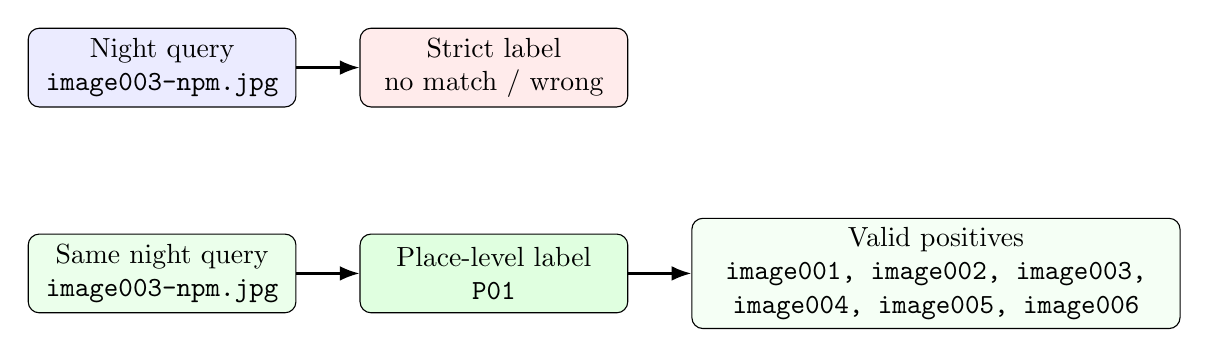
\begin{tikzpicture}[
  node distance=9mm and 8mm,
  box/.style={draw, rounded corners, align=center, minimum width=34mm, minimum height=10mm},
  arrow/.style={-{Latex[length=2.5mm]}, thick}
]
\node[box, fill=blue!8] (strictq) {Night query\\\code{image003-npm.jpg}};
\node[box, right=of strictq, fill=red!8] (strictgt) {Strict label\\no match / wrong};
\node[box, below=16mm of strictq, fill=green!8] (placeq) {Same night query\\\code{image003-npm.jpg}};
\node[box, right=of placeq, fill=green!12] (placegt) {Place-level label\\\code{P01}};
\node[box, right=of placegt, fill=green!4, minimum width=62mm] (multi) {Valid positives\\\code{image001, image002, image003,}\\\code{image004, image005, image006}};

\draw[arrow] (strictq) -- (strictgt);
\draw[arrow] (placeq) -- (placegt);
\draw[arrow] (placegt) -- (multi);
\end{tikzpicture}
\caption{The main relabeling idea: the same query moves from a strict image-level label to a place-level label with multiple valid daytime positives.}
\end{figure}

\subsection*{Example}
One concrete example is the query \code{image003-npm.jpg}. Under the original labeling it was treated as a no-match image. After visual inspection, it was clearly another night view of the \textbf{atrium central lobby}, so in the place-level dataset it is rematched to:
\begin{itemize}[leftmargin=*]
  \item \code{place\_id = P01}
  \item valid positives:
  \code{image001.jpg | image002.jpg | image003.jpg | image004.jpg | image005.jpg | image006.jpg}
\end{itemize}

So in the new evaluation, the query is counted as correct if the system retrieves \emph{any} valid daytime image from the same place.

\subsection*{What changed quantitatively}
The place-level relabeling produced:
\begin{itemize}[leftmargin=*]
  \item \textbf{64 place-level matched queries}
  \item \textbf{0 remaining no-match queries}
  \item \textbf{12 queries rematched from original \code{-npm} labels}
  \item \textbf{10 unique place IDs}
\end{itemize}

\begin{figure}[H]
\centering
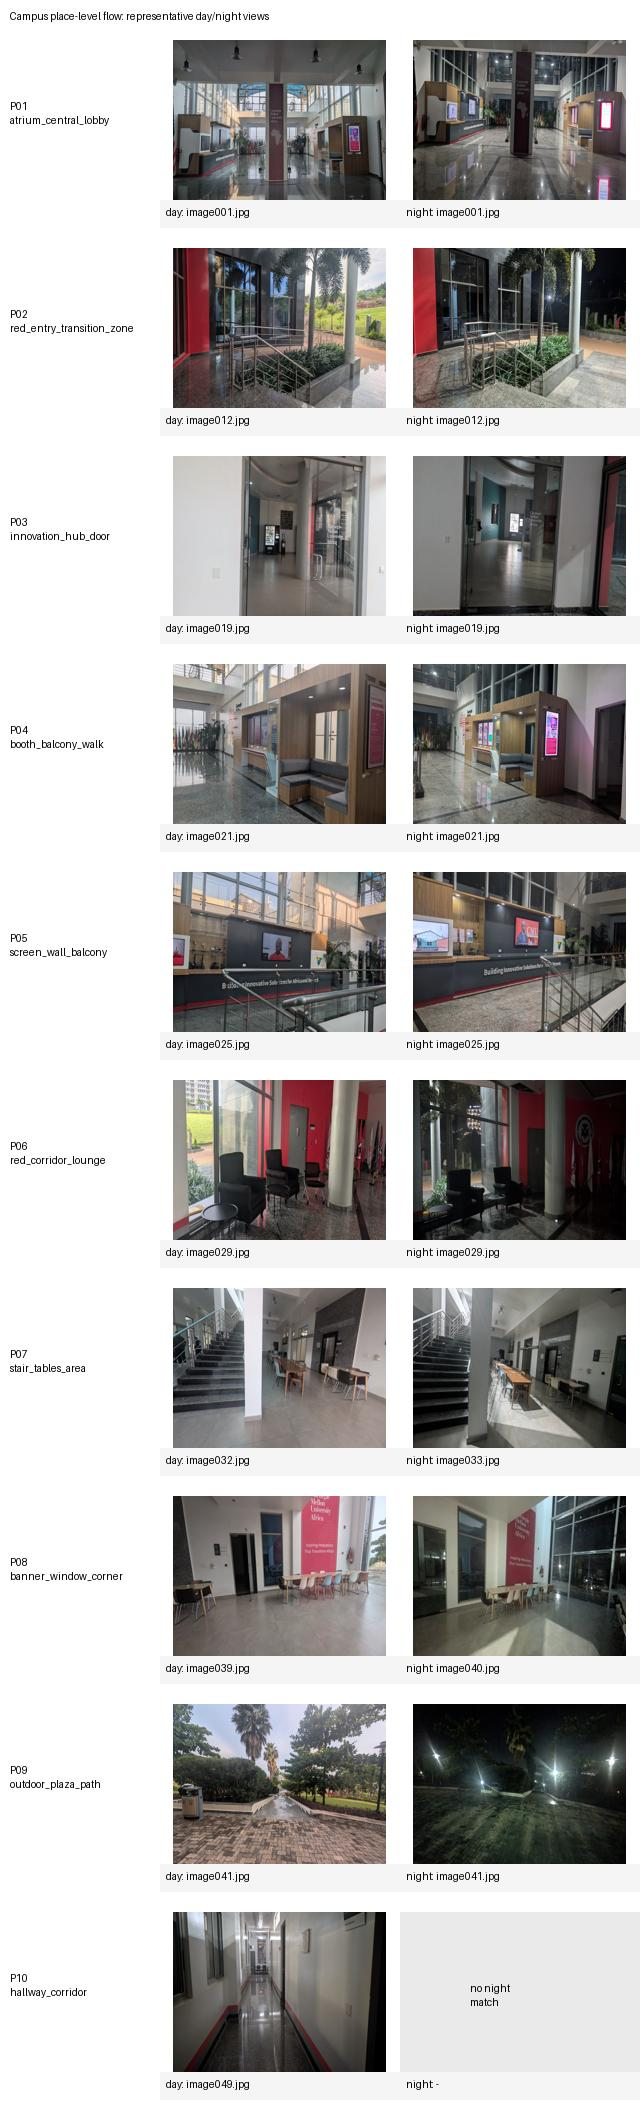
\includegraphics[width=0.92\textwidth]{../../custom_dataset_place_level/place_flow_visual.jpg}
\caption{Representative day/night views for the 10 manually defined place IDs in the place-level dataset.}
\end{figure}

\section{New Implementation}
To preserve the original evaluation path, we created new files rather than modifying the old ones:
\begin{itemize}[leftmargin=*]
  \item original loader: \file{datasets/load\_dataset.py} $\rightarrow$ \code{CampusDataset}
  \item new loader: \file{datasets/load\_dataset\_place\_level.py} $\rightarrow$ \code{CampusPlaceLevelDataset}
  \item original test script: \file{test\_campus\_dataset.py}
  \item new test script: \file{test\_campus\_dataset\_place\_level.py}
\end{itemize}

The new loader reads the CSV annotations and builds a \textbf{multi-positive} ground truth matrix:

\begin{lstlisting}[style=repo,language=Python,caption={Core idea of the place-level ground-truth construction.}]
valid_names = [
    part.strip()
    for part in row.get("valid_day_images", "").split("|")
    if part.strip()
]
for valid_name in valid_names:
    db_idx = day_lookup.get(valid_name)
    if db_idx is not None:
        gt[db_idx, q_idx] = True
\end{lstlisting}

So each query column can now contain \textbf{multiple true positives} instead of exactly one.

Importantly, the new test script still uses the same main evaluation flow:
\begin{itemize}[leftmargin=*]
  \item descriptor extraction,
  \item similarity matrix computation,
  \item thresholded matching,
  \item precision-recall,
  \item Recall@K.
\end{itemize}

That means the comparison between old and new results is still meaningful.

\section{Strict Image-Level Results}
\begin{table}[H]
\centering
\small
\begin{tabular}{L{2.4cm}C{1.0cm}C{1.1cm}C{0.9cm}C{0.9cm}C{0.9cm}}
\toprule
\textbf{Descriptor} & \textbf{AUC} & \textbf{R@100P} & \textbf{R@1} & \textbf{R@5} & \textbf{R@10} \\
\midrule
CosPlace    & 0.470 & 0.030 & 0.727 & 1.000 & 1.000 \\
EigenPlaces & 0.443 & 0.000 & 0.788 & 1.000 & 1.000 \\
NetVLAD     & 0.242 & 0.000 & 0.394 & 0.879 & 0.939 \\
AlexNet     & 0.512 & 0.061 & 0.758 & 0.939 & 0.939 \\
HDC-DELF    & 0.488 & 0.030 & 0.788 & 0.939 & 0.970 \\
SAD         & 0.106 & 0.000 & 0.212 & 0.545 & 0.727 \\
\bottomrule
\end{tabular}
\caption{Original strict image-level results from \file{test\_campus\_dataset.py}.}
\end{table}

\section{Place-Level Results}
\begin{table}[H]
\centering
\small
\begin{tabular}{L{2.4cm}C{1.0cm}C{1.1cm}C{0.9cm}C{0.9cm}C{0.9cm}}
\toprule
\textbf{Descriptor} & \textbf{AUC} & \textbf{R@100P} & \textbf{R@1} & \textbf{R@5} & \textbf{R@10} \\
\midrule
CosPlace     & 0.627 & 0.114 & 0.969 & 1.000 & 1.000 \\
EigenPlaces  & 0.663 & 0.110 & 0.922 & 1.000 & 1.000 \\
NetVLAD      & 0.512 & 0.024 & 0.891 & 0.938 & 0.969 \\
PatchNetVLAD & 0.641 & 0.074 & 0.938 & 1.000 & 1.000 \\
AlexNet      & 0.387 & 0.074 & 0.859 & 0.969 & 1.000 \\
HDC-DELF     & 0.507 & 0.132 & 0.922 & 0.969 & 0.984 \\
SAD          & 0.170 & 0.000 & 0.297 & 0.625 & 0.766 \\
\bottomrule
\end{tabular}
\caption{Place-level results from \file{test\_campus\_dataset\_place\_level.py}.}
\end{table}

\section{Direct Comparison}
\begin{table}[H]
\centering
\small
\begin{tabularx}{\textwidth}{L{2.2cm}C{1.2cm}C{1.4cm}C{1.1cm}Y}
\toprule
\textbf{Descriptor} & \textbf{$\Delta$ AUC} & \textbf{$\Delta$ R@100P} & \textbf{$\Delta$ R@1} & \textbf{Main effect} \\
\midrule
CosPlace    & +0.157 & +0.084 & +0.242 & Strong gain once same-place alternate views are credited. \\
EigenPlaces & +0.220 & +0.110 & +0.134 & Best overall AUC after relabeling. \\
NetVLAD     & +0.270 & +0.024 & +0.497 & Largest recovery in top-1, showing strict labels were penalizing it heavily. \\
AlexNet     & -0.125 & +0.013 & +0.101 & Better top-1, but weaker AUC under place-level evaluation. \\
HDC-DELF    & +0.019 & +0.102 & +0.134 & Much cleaner threshold behavior after relabeling. \\
SAD         & +0.064 & +0.000 & +0.085 & Improves slightly, but remains the weakest model. \\
\bottomrule
\end{tabularx}
\caption{Change from strict image-level evaluation to place-level evaluation.}
\end{table}

\section{Main Insights}
\subsection*{0. Main conclusion about the original setup}
We can now state the conclusion more clearly: the \textbf{original campus setup was not robust to multiple valid views under the original evaluation protocol}. In practice, that means:
\begin{itemize}[leftmargin=*]
  \item the descriptor pipeline was often retrieving the correct \emph{place},
  \item but the strict 1-to-1 image labels only credited one exact daytime image,
  \item so several correct same-place, different-view retrievals were counted as errors.
\end{itemize}

So the earlier weakness was not only a retrieval problem. It was also an \textbf{evaluation-design problem}. The place-level relabeling helps separate:
\begin{itemize}[leftmargin=*]
  \item truly wrong-place retrievals, from
  \item correct same-place retrievals that the original setup under-credited.
\end{itemize}

\subsection*{1. The relabeling changed the story substantially}
The place-level results confirm that the original dataset was indeed under-crediting correct retrievals. The clearest examples are:
\begin{itemize}[leftmargin=*]
  \item \textbf{CosPlace}: R@1 rises from \textbf{0.727} to \textbf{0.969}
  \item \textbf{EigenPlaces}: AUC rises from \textbf{0.443} to \textbf{0.663}
  \item \textbf{NetVLAD}: R@1 rises from \textbf{0.394} to \textbf{0.891}
\end{itemize}

This confirms that many earlier ``errors'' were not truly wrong places. They were often \textbf{same-place, different-view retrievals}.

\subsection*{2. EigenPlaces and CosPlace remain the strongest overall retrievers}
Under the place-level protocol:
\begin{itemize}[leftmargin=*]
  \item \textbf{CosPlace} gives the best \textbf{R@1 = 0.969}
  \item \textbf{EigenPlaces} gives the best \textbf{AUC = 0.663}
  \item both keep \textbf{R@5 = 1.000} and \textbf{R@10 = 1.000}
\end{itemize}

So the broad conclusion from the earlier benchmark remains true, but it is now supported by a fairer labeling protocol.

\subsection*{3. PatchNetVLAD becomes much more credible at place level}
PatchNetVLAD was not part of the original comparison table, but in the place-level evaluation it performs strongly:
\begin{itemize}[leftmargin=*]
  \item \textbf{AUC = 0.641}
  \item \textbf{R@1 = 0.938}
  \item \textbf{R@5 = 1.000}
\end{itemize}

This suggests PatchNetVLAD benefits from being evaluated on actual place consistency rather than exact image duplication.

\subsection*{4. AlexNet does not benefit as much as the others}
AlexNet improves in \textbf{R@1}, but its place-level \textbf{AUC} drops from \textbf{0.512} to \textbf{0.387}. So while it still gives a decent top-1 rate, it is no longer the most appealing option once the relabeling issue is corrected.

\subsection*{5. HDC-DELF looks more stable after relabeling}
Previously HDC-DELF looked noisy because many thresholded matches were marked as false positives. Under the place-level protocol:
\begin{itemize}[leftmargin=*]
  \item \textbf{R@100P} rises from \textbf{0.030} to \textbf{0.132}
  \item the printed threshold statistics no longer show false positives in the current run
\end{itemize}

So HDC-DELF appears more reasonable once same-place alternative views are credited correctly.

\subsection*{6. SAD remains weak}
SAD improves slightly, but it is still clearly the weakest descriptor in both protocols.

\section{How To Interpret the New Metrics}
The place-level evaluation is better aligned with real localization, but it is also important to recognize what changed:
\begin{itemize}[leftmargin=*]
  \item there are now \textbf{0 remaining unmatched queries},
  \item so the new benchmark is no longer testing open-set rejection in the same way,
  \item instead, it is mainly testing \textbf{place-level retrieval quality}.
\end{itemize}

So the two protocols serve different purposes:
\begin{itemize}[leftmargin=*]
  \item \textbf{strict image-level benchmark}: harsher, but still useful for exact pair evaluation
  \item \textbf{place-level benchmark}: better for real localization quality
\end{itemize}

\section{What This Means for the Project}
The main conclusion is now clearer:
\begin{itemize}[leftmargin=*]
  \item the campus benchmark was not just exposing descriptor weakness,
  \item it was also exposing a \textbf{ground-truth mismatch} between image-level labels and place-level localization.
\end{itemize}

After correcting that mismatch, the strongest methods are:
\begin{itemize}[leftmargin=*]
  \item \textbf{CosPlace}: strongest top-1 retrieval
  \item \textbf{EigenPlaces}: strongest overall AUC
  \item \textbf{PatchNetVLAD}: strong additional option for place-level retrieval
\end{itemize}

\section{Recommended Next Steps}
\begin{enumerate}[leftmargin=*]
  \item Keep \textbf{both} evaluation paths in the repo:
  \begin{itemize}[leftmargin=*]
    \item strict image-level for comparison with the original protocol
    \item place-level for realistic localization analysis
  \end{itemize}
  \item Use the \textbf{place-level benchmark} when arguing about real retrieval quality.
  \item Use the \textbf{strict benchmark} carefully, mainly to show how much the labeling assumption matters.
  \item If open-set rejection still matters, add a third benchmark split with truly unmatched night queries that remain unmatched even after place-level review.
  \item For the live demo, prioritize \textbf{CosPlace}, \textbf{EigenPlaces}, or \textbf{PatchNetVLAD}.
\end{enumerate}

\section*{Bottom Line}
The place-level relabeling was worth doing. It shows that the original campus setup was \textbf{not robust to multiple valid views under a strict image-level evaluation}, because it forced a 1-to-1 image correspondence where the real task is \textbf{place recognition across viewpoint changes}. After the relabeling, the strongest descriptors improve substantially, especially CosPlace, EigenPlaces, NetVLAD, and HDC-DELF. The project can now report a much fairer campus evaluation while still keeping the original strict benchmark for comparison.

\end{document}
